\PassOptionsToPackage{unicode=true}{hyperref} % options for packages loaded elsewhere
\PassOptionsToPackage{hyphens}{url}
%
\documentclass[]{article}
\usepackage{lmodern}
\usepackage{amssymb,amsmath}
\usepackage{ifxetex,ifluatex}
\usepackage{fixltx2e} % provides \textsubscript
\ifnum 0\ifxetex 1\fi\ifluatex 1\fi=0 % if pdftex
  \usepackage[T1]{fontenc}
  \usepackage[utf8]{inputenc}
  \usepackage{textcomp} % provides euro and other symbols
\else % if luatex or xelatex
  \usepackage{unicode-math}
  \defaultfontfeatures{Ligatures=TeX,Scale=MatchLowercase}
\fi
% use upquote if available, for straight quotes in verbatim environments
\IfFileExists{upquote.sty}{\usepackage{upquote}}{}
% use microtype if available
\IfFileExists{microtype.sty}{%
\usepackage[]{microtype}
\UseMicrotypeSet[protrusion]{basicmath} % disable protrusion for tt fonts
}{}
\IfFileExists{parskip.sty}{%
\usepackage{parskip}
}{% else
\setlength{\parindent}{0pt}
\setlength{\parskip}{6pt plus 2pt minus 1pt}
}
\usepackage{hyperref}
\hypersetup{
            pdftitle={Informe 3},
            pdfauthor={Derek Corcoran, Giorgia Graells, Horacio Samaniego, Pablo Marquet},
            pdfborder={0 0 0},
            breaklinks=true}
\urlstyle{same}  % don't use monospace font for urls
\usepackage[margin=1in]{geometry}
\usepackage{longtable,booktabs}
% Fix footnotes in tables (requires footnote package)
\IfFileExists{footnote.sty}{\usepackage{footnote}\makesavenoteenv{longtable}}{}
\usepackage{graphicx,grffile}
\makeatletter
\def\maxwidth{\ifdim\Gin@nat@width>\linewidth\linewidth\else\Gin@nat@width\fi}
\def\maxheight{\ifdim\Gin@nat@height>\textheight\textheight\else\Gin@nat@height\fi}
\makeatother
% Scale images if necessary, so that they will not overflow the page
% margins by default, and it is still possible to overwrite the defaults
% using explicit options in \includegraphics[width, height, ...]{}
\setkeys{Gin}{width=\maxwidth,height=\maxheight,keepaspectratio}
\setlength{\emergencystretch}{3em}  % prevent overfull lines
\providecommand{\tightlist}{%
  \setlength{\itemsep}{0pt}\setlength{\parskip}{0pt}}
\setcounter{secnumdepth}{5}
% Redefines (sub)paragraphs to behave more like sections
\ifx\paragraph\undefined\else
\let\oldparagraph\paragraph
\renewcommand{\paragraph}[1]{\oldparagraph{#1}\mbox{}}
\fi
\ifx\subparagraph\undefined\else
\let\oldsubparagraph\subparagraph
\renewcommand{\subparagraph}[1]{\oldsubparagraph{#1}\mbox{}}
\fi

% set default figure placement to htbp
\makeatletter
\def\fps@figure{htbp}
\makeatother

\usepackage{booktabs}
\usepackage{longtable}
\usepackage{array}
\usepackage{multirow}
\usepackage{wrapfig}
\usepackage{float}
\usepackage{colortbl}
\usepackage{pdflscape}
\usepackage{tabu}
\usepackage{threeparttable}
\usepackage{threeparttablex}
\usepackage[normalem]{ulem}
\usepackage{makecell}
\usepackage{xcolor}

\title{Informe 3}
\author{Derek Corcoran, Giorgia Graells, Horacio Samaniego, Pablo Marquet}
\date{20/04/2020}

\begin{document}
\maketitle

\hypertarget{introducciuxf3n}{%
\section{Introducción}\label{introducciuxf3n}}

En este documento se mostrarán simulaciones destinadas a responder 3 puntos de la minuta solicitados por el ministerio de ciencia, basado en un modelo con conectividad espacial y estrucutrado por edades (Arenas et al. 2020), la modificación del modelo se encuentra explicada en detalle en Corcoran et al. (2020)

\begin{enumerate}
\def\labelenumi{\arabic{enumi}.}
\item
  Cuarentena total, las personas quedan con prohibición de salir de su casa, solo con permiso especiales.
\item
  Cuarentenas alternantes por comunas a nivel nacional de 15 días, las personas quedan con prohibición de salir de su casa 15 días (cuarentena) y luego 15 días con cierre de colegios y comercio. Una comuna entra en cuarentena cuando los casos llegan a 4 o 5 por 10.000.
\item
  Cierre de colegios y comercio.
\end{enumerate}

\hypertarget{simulaciones}{%
\section{Simulaciones}\label{simulaciones}}

Para todas las simulaciones se usaron el las funciones descritas y disponibles en Corcoran and Graells (2020), ahí también se encuentran las bases de datos con las que se realizaron estas simulaiciones

\hypertarget{cuarentena-nacional-total}{%
\subsection{Cuarentena Nacional total}\label{cuarentena-nacional-total}}

\hypertarget{extensiuxf3n-uxf3ptima-de-cuarentena-total.-simulaciuxf3n-del-15-abril-al-14-junio}{%
\subsubsection{Extensión óptima de cuarentena total. Simulación del 15 abril al 14 junio}\label{extensiuxf3n-uxf3ptima-de-cuarentena-total.-simulaciuxf3n-del-15-abril-al-14-junio}}

Para obtener la extensión óptima de una cuarentena total a nivel nacional se realizaron 12 simulaciones distintas que parten el día 20 de abril. Se consideraron 3 extensiones de cuarentena nacional (7, 15 y 30 días) y 3 valores de grado de confinamiento o \(\kappa_0\) distintos (0.5, 0.75 y 0.85, cada una representando cuarentenas con control leve, medio o fuerte). Para tener las condiciones iniciales del 20 de abril se modeló del 15 abril al 20 abril, manteniendo una cuarentena dinámica por comuna.

Estas simulaciones se contrastaron con una cuarentena dinámica la cual se gatilla cuando el número de infectados llega a 40/100,000 casos activos confirmados. Una vez gatillada la cuarentena, esta durará como mínimo 7 días, y al pasar los 7 días se observa la prevalencia nuevamente para determinar si la cuarentena se levanta o se renueva por otros 7 días

\hypertarget{inicio-uxf3ptimo-de-cuarentena-total.-simulaciuxf3n-del-15-abril-al-14-junio}{%
\subsubsection{Inicio óptimo de cuarentena total. Simulación del 15 abril al 14 junio}\label{inicio-uxf3ptimo-de-cuarentena-total.-simulaciuxf3n-del-15-abril-al-14-junio}}

Extendiendo el ejercicio anterior se probaron cuarentenas nacionales con cuarentenas fuertes y medias empezando en los días 20 de Abril, 27 de Abril y 4 de mayo, con extenciones de 15 y 30 días, para medir el efecto del inicio de la fecha de cuarentena

\hypertarget{resultados}{%
\section{Resultados}\label{resultados}}

\hypertarget{cuarentena-nacional-total-1}{%
\subsection{Cuarentena Nacional total}\label{cuarentena-nacional-total-1}}

\hypertarget{extensiuxf3n-uxf3ptima-de-cuarentena-total}{%
\subsubsection{Extensión óptima de cuarentena total}\label{extensiuxf3n-uxf3ptima-de-cuarentena-total}}

Si observamos los resultados para la totalidad de la región para el número de infectados activos figuras \ref{fig:InfectadosRM} y \ref{fig:UCIRM} vemos que cuando empezamos cuarentenas nacionales el día 20 de abril por 7, 15 o 30 días, el comportamiento de el número mas altó de infectados y de pacientes en Unidad de Cuidado Intensivo variarán dependiendo de la intensidad de la cuarentena. Cuanto mas fuerte sea la cuarentena mas se desplaza el peak de la curva hacia al futuro. Sin embargo en el caso de las Cuarentenas nacionales, esto no disminuye el peak de la curva notoriamente, salvo en el caso del lockdown nacional de 30 días con cuarentena leve.

\begin{figure}
\centering
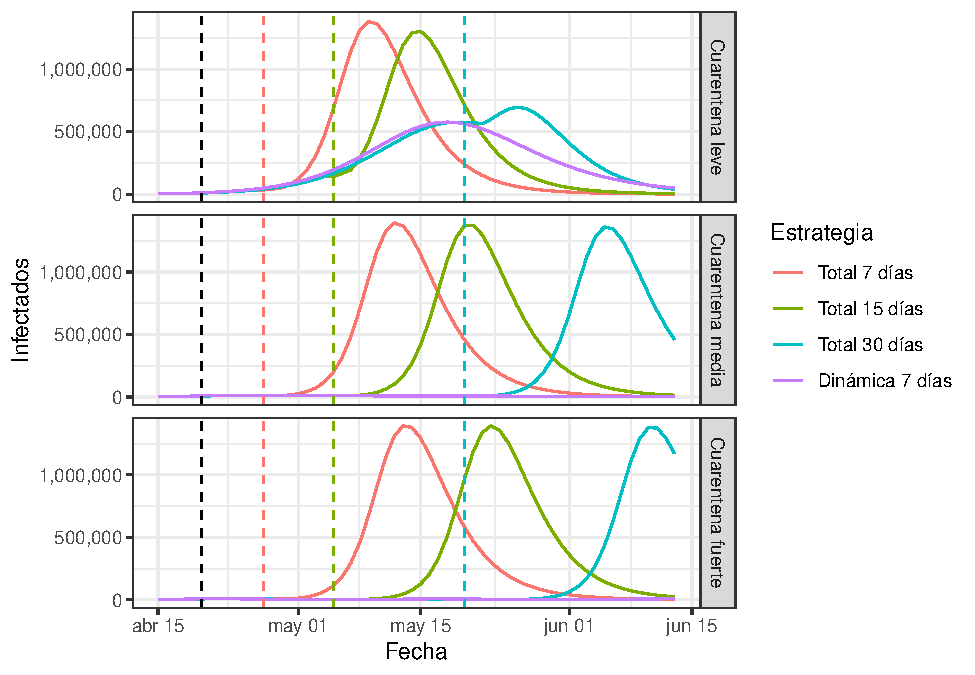
\includegraphics{Informe_Mesa_2020_04_16_files/figure-latex/InfectadosRM-1.pdf}
\caption{\label{fig:InfectadosRM}Evolución de número de infectados en el tiempo en la Región Metropolitana, dadas distintas estrategias, la linea punteada negra es la fecha en que parte la cuarentena nacional para todas las Cuarentenas totales, las lineas roja, verde y azul representan cuando terminan las cuarentenas totales de 7, 15 y 30 días respectivamente}
\end{figure}

\begin{figure}
\centering
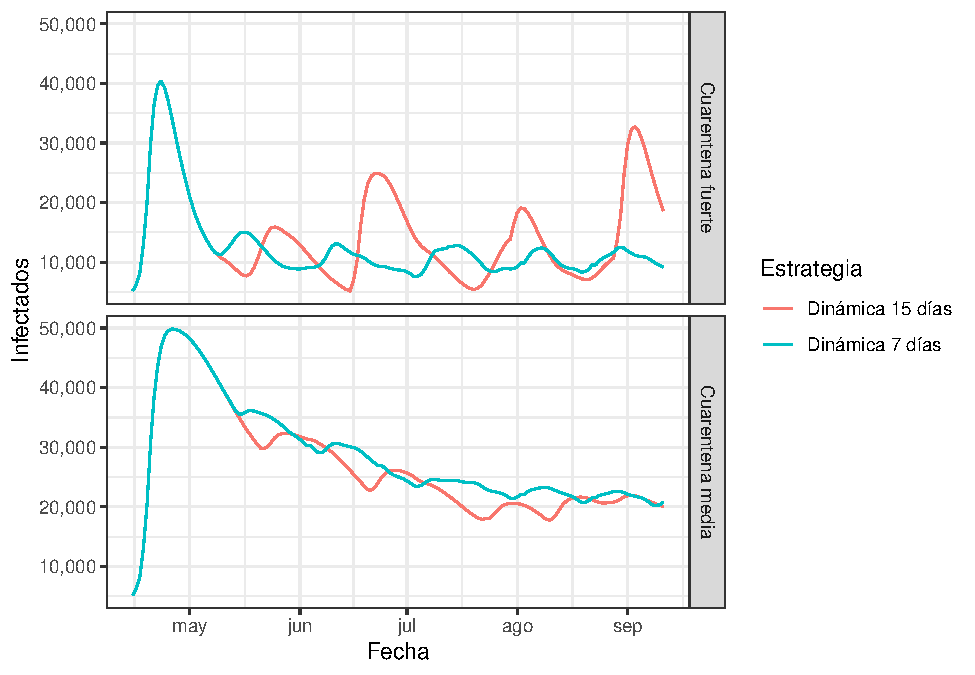
\includegraphics{Informe_Mesa_2020_04_16_files/figure-latex/InfectadosRMDin-1.pdf}
\caption{\label{fig:InfectadosRMDin}Evolución de número de infectados en el tiempo en la Región Metropolitana, dadas distintas estrategias}
\end{figure}

\begin{figure}
\centering
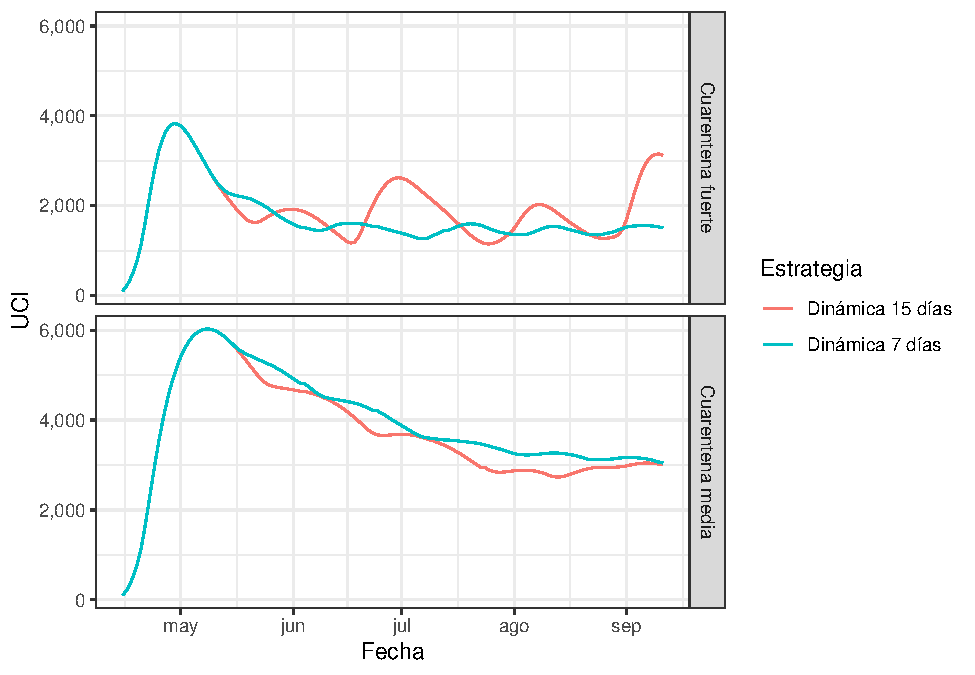
\includegraphics{Informe_Mesa_2020_04_16_files/figure-latex/UCIRMDin-1.pdf}
\caption{\label{fig:UCIRMDin}Evolución de número de infectados en el tiempo en la Región Metropolitana, dadas distintas estrategias}
\end{figure}

Al tener una cuarentena de 30 días con de cuarentena leve, el lecantamiento de esta coincide con un momento posterior al peak de infectados como se ve en la figura \ref{fig:InfectadosRM}, esto parece ser que es lo que rompe el equilibrio, que la cuarentena termine después del peak.

Esto se traduce tambien en una disminución fuerte en el número mas alto de personas que requerirán de estar Hospitalizadas en Unidades de Cuidado Intensivo (figura \ref{fig:UCIRM}).

\begin{figure}
\centering
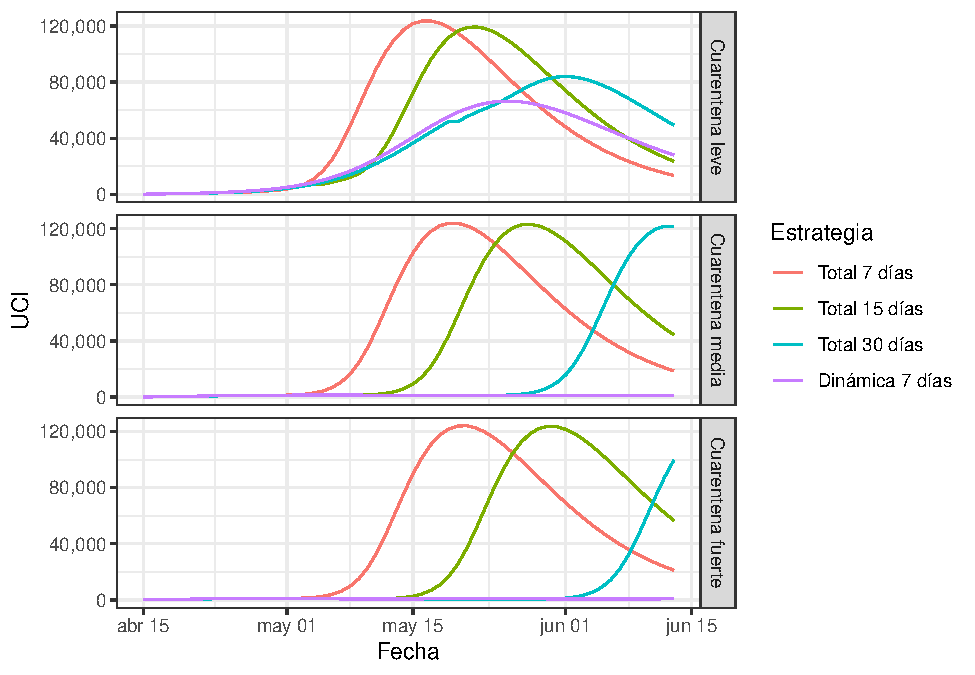
\includegraphics{Informe_Mesa_2020_04_16_files/figure-latex/UCIRM-1.pdf}
\caption{\label{fig:UCIRM}Evolución de número de pacientes en unidad de Cuidado Intensivo en el tiempo en la Región Metropolitana, dadas distintas estrategias, la linea punteada negra es la fecha en que parte la cuarentena nacional para todas las Cuarentenas totales, las lineas roja, verde y azul representan cuando terminan las cuarentenas totales de 7, 15 y 30 días respectivamente}
\end{figure}

Al ver el comportamiento de la cuarentena adaptativa en la figura \ref{fig:InfectadosRM}, uno podría pensar que es mas conveniente el realizar una cuarentena adaptativa mas que una cuarentena nacional, Sin embargo, la cuarentena adaptativa implica muchos más días totales en cuarentena, y generar una cuarentena mucho más intensa como vemos en la tabla \ref{tab:DiasCuar}

\begin{table}

\caption{\label{tab:DiasCuar}Numero de días promedio de cuarentena según estrategia e intensidad de cuarentena}
\centering
\begin{tabular}[t]{llrr}
\toprule
Estrategia & Intensidad de Cuarentena & Días promedio & Desviacion\\
\midrule
Total 7 días & Cuarentena leve & 10.2 & 1.5\\
Total 7 días & Cuarentena media & 10.2 & 1.6\\
Total 7 días & Cuarentena fuerte & 10.2 & 1.6\\
Total 15 días & Cuarentena leve & 18.2 & 1.5\\
Total 15 días & Cuarentena media & 18.2 & 1.6\\
\addlinespace
Total 15 días & Cuarentena fuerte & 18.2 & 1.6\\
Total 30 días & Cuarentena leve & 33.2 & 1.5\\
Total 30 días & Cuarentena media & 33.2 & 1.6\\
Total 30 días & Cuarentena fuerte & 33.2 & 1.6\\
Dinámica 7 días & Cuarentena leve & 58.2 & 1.7\\
\addlinespace
Dinámica 7 días & Cuarentena media & 141.2 & 8.8\\
Dinámica 7 días & Cuarentena fuerte & 49.7 & 3.9\\
Dinámica 15 días & Cuarentena leve & 90.6 & 9.8\\
Dinámica 15 días & Cuarentena media & 141.0 & 8.1\\
Dinámica 15 días & Cuarentena fuerte & 125.7 & 8.0\\
\bottomrule
\end{tabular}
\end{table}

\hypertarget{nivel-comunal-regiuxf3n-metropolitana}{%
\subsection{Nivel Comunal Región Metropolitana}\label{nivel-comunal-regiuxf3n-metropolitana}}

\begin{figure}
\centering
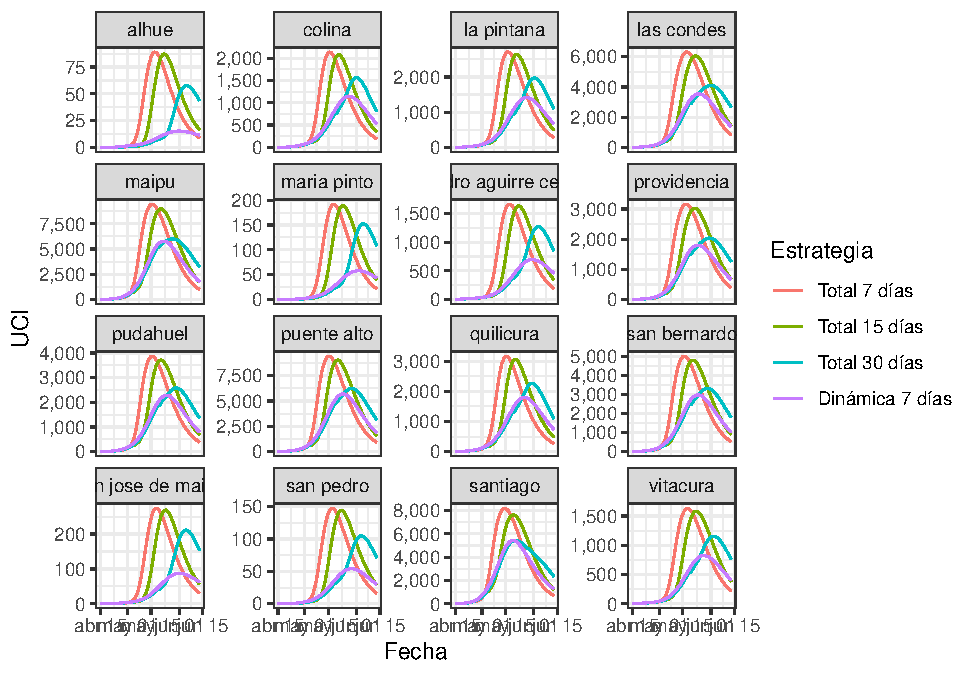
\includegraphics{Informe_Mesa_2020_04_16_files/figure-latex/UCIComunal-1.pdf}
\caption{\label{fig:UCIComunal}Evolución de número de pacientes en unidad de Cuidado Intensivo en el tiempo en comunas de la Región Metropolitana, dadas distintas estrategias, la linea punteada negra es la fecha en que parte la cuarentena nacional para todas las Cuarentenas totales, las lineas roja, verde y azul representan cuando terminan las cuarentenas totales de 7, 15 y 30 días respectivamente}
\end{figure}

\hypertarget{inicio-uxf3ptimo-de-cuarentena-total}{%
\subsubsection{Inicio óptimo de cuarentena total}\label{inicio-uxf3ptimo-de-cuarentena-total}}

\begin{figure}
\centering
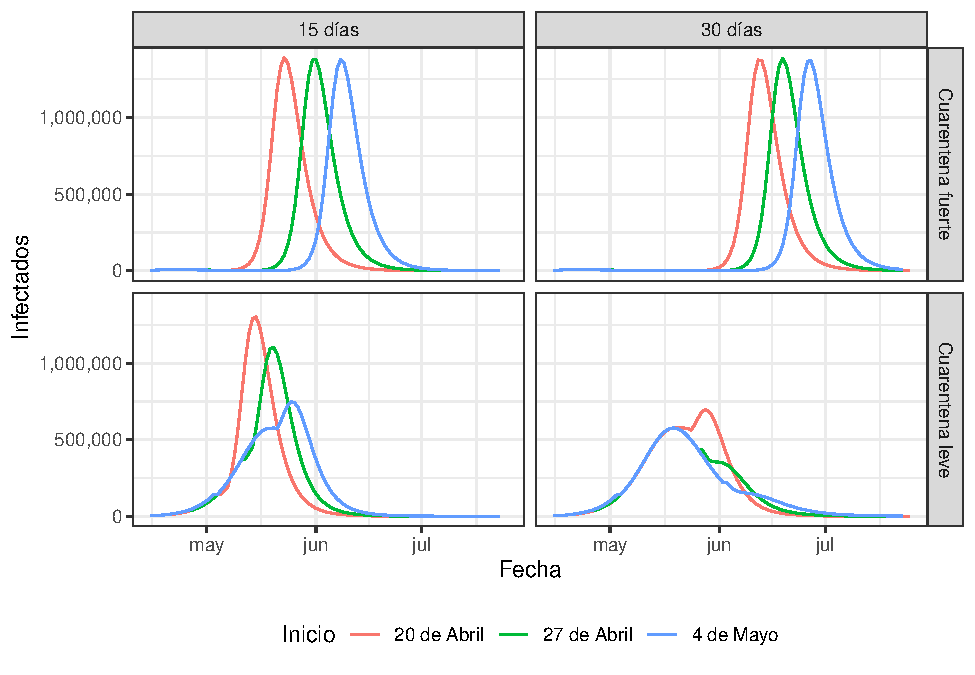
\includegraphics{Informe_Mesa_2020_04_16_files/figure-latex/InicioDuracion-1.pdf}
\caption{\label{fig:InicioDuracion}Efecto de la fecha de inicio, duración de cuarentena y número de días de la cuarentena Nacional}
\end{figure}

\begin{figure}
\centering
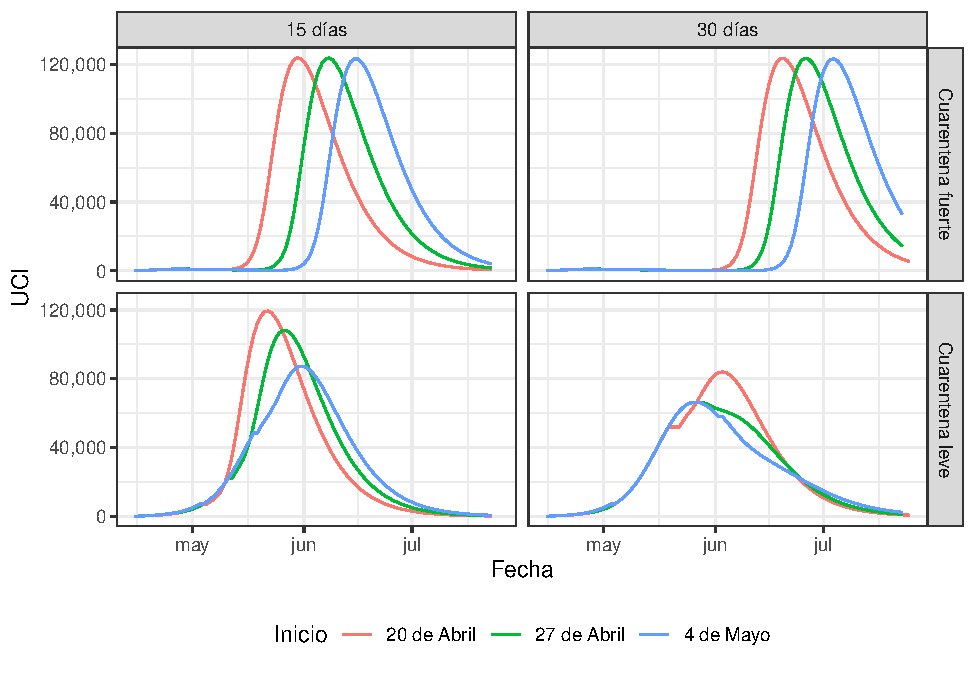
\includegraphics{Informe_Mesa_2020_04_16_files/figure-latex/InicioDuracionUCI-1.pdf}
\caption{\label{fig:InicioDuracionUCI}Efecto de la fecha de inicio, duración de cuarentena y número de días de la cuarentena Nacional en el número de pacientes de Estado Crítico}
\end{figure}

\begin{table}

\caption{\label{tab:DiasCuar2}Numero de días promedio de cuarentena según estrategia e intensidad de cuarentena}
\centering
\begin{tabular}[t]{lllrr}
\toprule
Intensidad cuarentena & Inicio & Duracion & Dias promedio & Desviación\\
\midrule
Cuarentena fuerte & 20 de Abril & 15 días & 18.2 & 1.6\\
Cuarentena leve & 20 de Abril & 15 días & 18.2 & 1.5\\
Cuarentena fuerte & 27 de Abril & 15 días & 25.1 & 1.7\\
Cuarentena leve & 27 de Abril & 15 días & 25.2 & 1.7\\
Cuarentena fuerte & 4 de Mayo & 15 días & 31.2 & 1.9\\
\addlinespace
Cuarentena leve & 4 de Mayo & 15 días & 32.2 & 1.7\\
Cuarentena fuerte & 20 de Abril & 30 días & 33.2 & 1.6\\
Cuarentena leve & 20 de Abril & 30 días & 33.2 & 1.5\\
Cuarentena fuerte & 27 de Abril & 30 días & 40.1 & 1.7\\
Cuarentena leve & 27 de Abril & 30 días & 40.2 & 1.7\\
\addlinespace
Cuarentena fuerte & 4 de Mayo & 30 días & 46.2 & 1.9\\
Cuarentena leve & 4 de Mayo & 30 días & 47.2 & 1.7\\
\bottomrule
\end{tabular}
\end{table}

\hypertarget{recomendaciones}{%
\section{Recomendaciones}\label{recomendaciones}}

Considerando tanto los peaks, la estrategia más adecuada según las simulaciones entregadas sería el empezar con una cuarentena leve a nivel nacional por 15 días desde el lunes 04 de Mayo, realizandose una cuarentena dinámica antes de llegar a esa fecha. Esta estrategia reduce de forma significativa el peak de infectados y de pacientes que necesitarán del uso de Unidades de Cuidado Intensivo. Considerando los días de cuarentena (cuarentena adaptativa y cuarentena total), esta estrategia necesita una menor cantidad de días totales para disminuir el número de afectados (ver tablas \ref{tab:DiasCuar} y \ref{tab:DiasCuar2}).

En terminos prácticos, una cuarentena menos estricta, implica una cuarentena similar a la actual, donde en lo posible continuamos con distanciamiento social, establecimientos de eduacación cerrados, con teletrabajo. Dado que todos estas simulaciones consideraron movilidad muy reducida del grupo de menores de 25 años, esto tuvo en todo momento considerado el no tener clases presenciales.

\hypertarget{referencias}{%
\section*{Referencias}\label{referencias}}
\addcontentsline{toc}{section}{Referencias}

\hypertarget{refs}{}
\leavevmode\hypertarget{ref-arenas2020mathematical}{}%
Arenas, Alex, Wesley Cota, Jesus Gomez-Gardenes, Sergio Gómez, Clara Granell, Joan T Matamalas, David Soriano-Panos, and Benjamin Steinegger. 2020. ``A Mathematical Model for the Spatiotemporal Epidemic Spreading of Covid19.'' \emph{medRxiv}. Cold Spring Harbor Laboratory Press.

\leavevmode\hypertarget{ref-derek_corcoran_barrios_2020_3756847}{}%
Corcoran, Derek, and Giorgia Graells. 2020. \emph{derek-corcoran-barrios/Covid19\_Chile\_Age: Modelo metapoblacional para simular el manejo de COVID19 en Chile} (version V1.0). Zenodo. \url{https://doi.org/10.5281/zenodo.3756847}.

\leavevmode\hypertarget{ref-corcoran_graells_2020}{}%
Corcoran, Derek, Giorgia Graells, Simón Castillo, Horacio Samaniego, and Pablo Marquet. 2020. ``Mplementación de Modelo Covid19 paraChile.'' \emph{Ecoinformatica}. \url{https://www.ecoinformatica.net/COVID19.html}.

\end{document}
